Da der Schwerpunkt dieser Arbeit auf dem Umgang mit Konflikten der zu testenden offlineunterstützenden Technologien liegt, soll die Bedienoberfläche der Anwendung möglichst einfach gehalten werden.\\
Alle Adressbucheinträge sollen in einer Liste angezeigt werden. Zum Anlegen, Editieren und Löschen eines einzelnen Eintrags soll es eine zweite Ansicht geben, auf die man per Klick auf den entsprechenden Eintrag in der Liste gelangt.
Wenn es zum Konflikt kommt, kann dieser über ein Dialogfenster aufgelöst werden. Im Dialog muss erkennbar sein wo, bei welchem Kontakteintrag, der Konflikt auftrat.
Außerdem müssen sich die entsprechenden Bereiche beider Versionen unterscheiden lassen und auswählbar sein. \autoref{fig:dialog} zeigt wie so ein Dialogfenster aussehen könnte.
\begin{figure}[H]
	\centering
	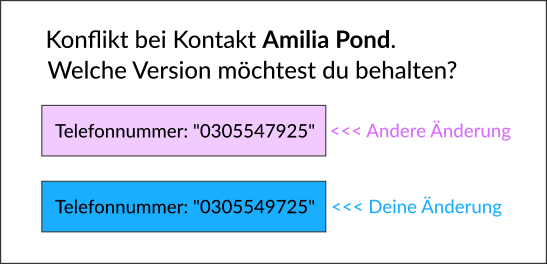
\includegraphics[width=0.8\textwidth]{Konfliktdialog}
	\grayRule
	\caption{Dialogfenster im Konfliktfall}
	\label{fig:dialog}
\end{figure}
Wurde beispielsweise Amilias Telefonnummer von zwei Personen gleichzeitig bearbeitet, bildet der Dialog zwei Bereiche mit der Nummer in den unterschiedlichen Versionen ab. Daneben ist abzulesen woher die Änderung kommt.
Durch Klick auf die korrekte Nummer kann entschieden werden welche Version die richtige ist und behalten wird.